% 2007 年上海卷文科第 7 题：直三棱柱示意图。
% 保留 A1B 斜线、直角顶点 C、虚线底棱 AC/CB 与隐藏棱 CC1；比例按原图示意。
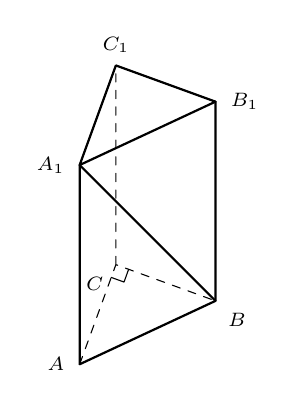
\begin{tikzpicture}[x=1.15cm,y=1.15cm,line cap=round,line join=round,
  every node/.style={font=\scriptsize}]
  \coordinate (A)  at (0,0);
  \coordinate (C)  at (.4,1.1);
  \coordinate (B)  at (1.5,.7);
  \coordinate (A1) at (0,2.2);
  \coordinate (C1) at (.4,3.3);
  \coordinate (B1) at (1.5,2.9);

  % 隐藏底边与后侧棱先画，随后覆盖可见斜线。
  \draw[dashed] (A)--(C)--(B) (C)--(C1);
  \draw[thick] (A)--(B) (A)--(A1) (B)--(B1);
  \draw[thick] (A1)--(C1)--(B1)--cycle;
  \draw[thick] (A1)--(B);

  % C 处为直角，符号按透视示意绘出。
  \draw[line width=.4pt] (.349,.959)--(.49,.908)--(.541,1.049);

  \node[left=2pt] at (A) {$A$};
  \node[below right=1pt] at (B) {$B$};
  \node[below left=1pt] at (C) {$C$};
  \node[left=2pt] at (A1) {$A_1$};
  \node[above=1pt] at (C1) {$C_1$};
  \node[right=2pt] at (B1) {$B_1$};
\end{tikzpicture}
